% !TEX encoding = UTF-8
% !TEX TS-program = pdflatex
% !TEX root = ../tesi.tex

%**************************************************************
\chapter{Analisi del contesto aziendale}
\label{cap:analisi-del-contesto-aziendale}
%**************************************************************

%Introduzione al contesto applicativo.\\

%\noindent Esempio di utilizzo di un termine nel glossario \\
%\gls{api}. \\

%\noindent Esempio di citazione in linea \\
%\cite{site:agile-manifesto}. \\

%\noindent Esempio di citazione nel pie' di pagina \\
%citazione\footcite{womak:lean-thinking} \\

%**************************************************************

\section{L'azienda San Marco Group}

San Marco Group è un gruppo aziendale \textit{leader} in Italia nella produzione di pitture e vernici per l'edilizia professionale. Il gruppo con sede principale a Marcon (VE) conta 300 dipendenti, è proprietario di 7 diversi \textit{brand}, ha un fatturato pari a 80 milioni di euro ed una rete distributiva che tocca oltre 100 Paesi. Tutti i prodotti vengono progettati negli stabilimenti italiani, mentre la produzione si divide tra Italia, Bosnia e Russia, con un totale di 8 stabilimenti produttivi che producono per tutti i \textit{brand} del gruppo. La sede di Marcon ospita 150 dipendenti, tra impiegati e operai, e vi si trovano gli uffici delle funzioni centrali del gruppo, unità produttive e magazzini. \\
I prodotti San Marco vengono distribuiti attraverso un \textit{network} di rivenditori specializzati in Italia e all'estero, e in esclusiva per il mercato italiano attraverso il primo \textit{marketplace} di proprietà dedicato alle pitture.

\vspace{10pt}
\begin{figure}[htbp]
	\begin{center}
		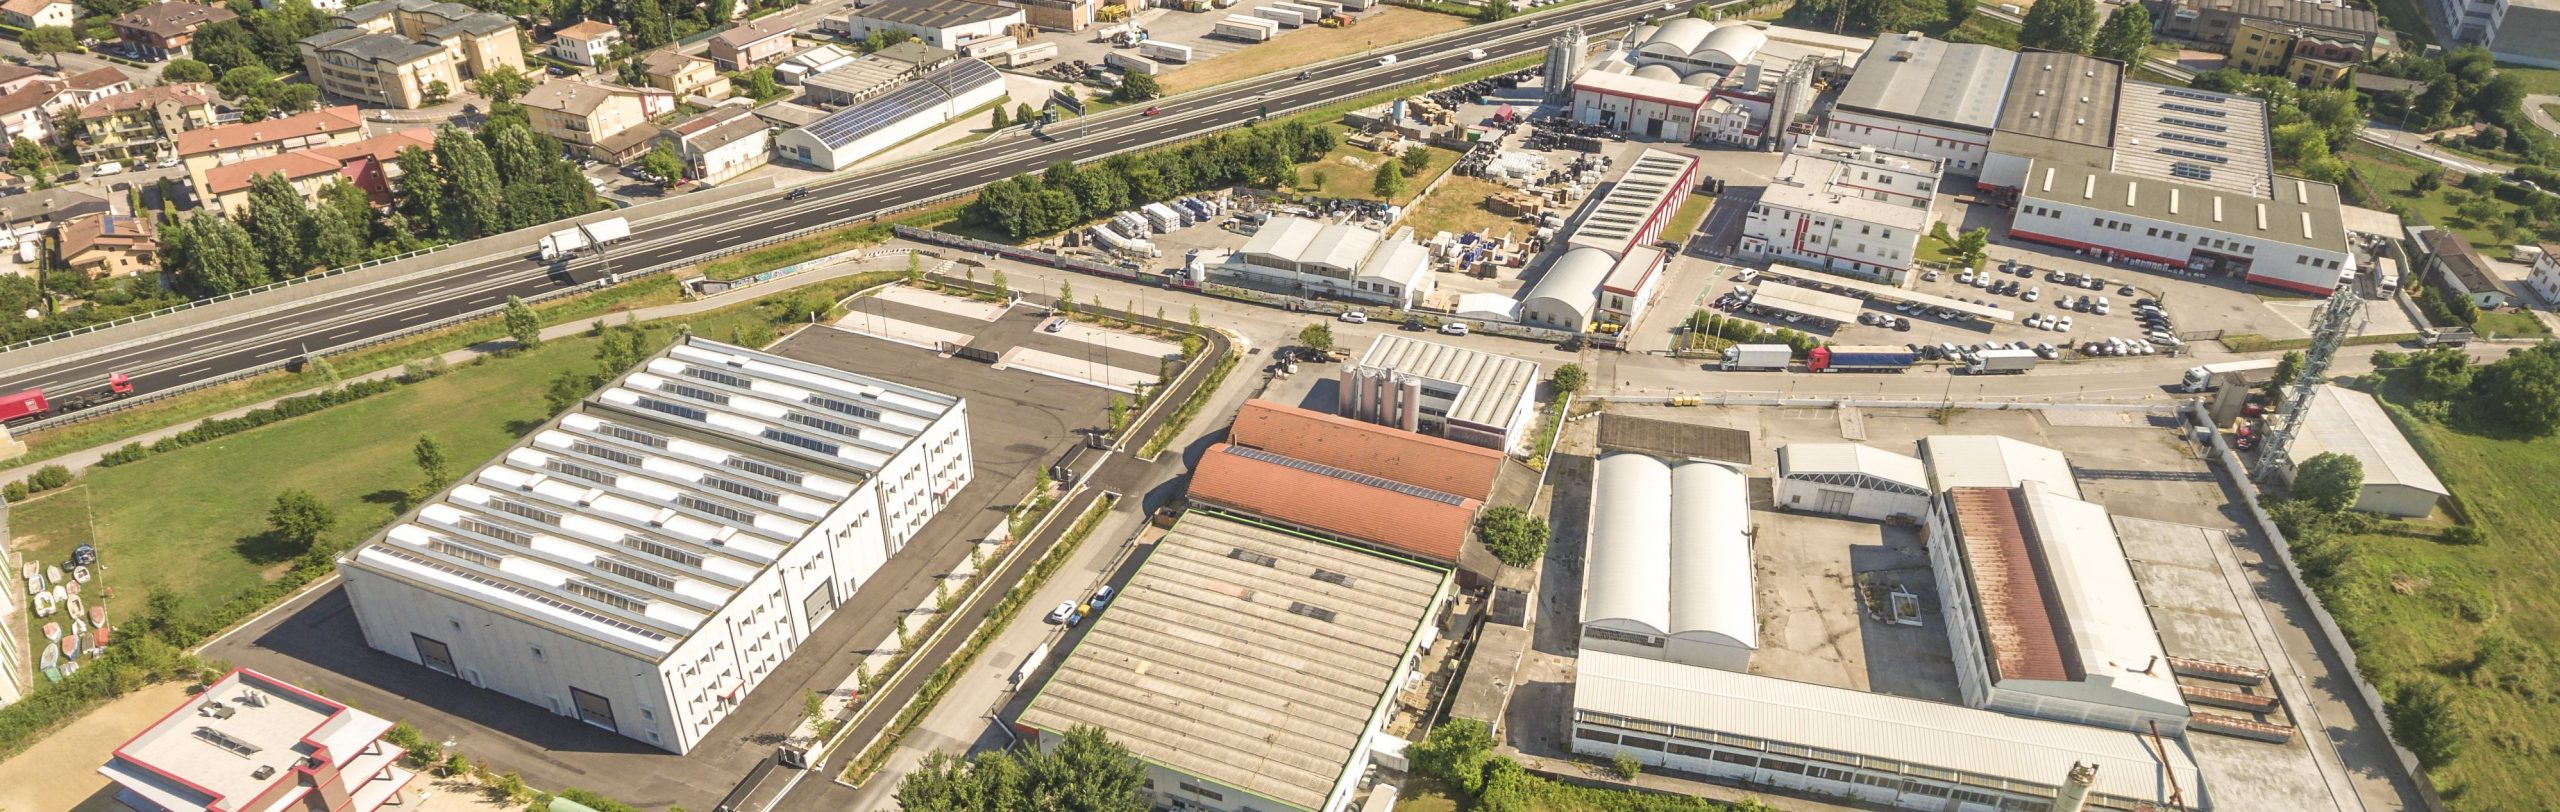
\includegraphics[height=4.2cm]{sede-marcon}
		\caption{Sede principale di Marcon (VE). \newline \textbf{Fonte: }\url{https://sanmarcogroup.com/}}
	\end{center}
\end{figure}
\vspace{10pt}

La gamma di prodotti offerti dall'azienda riesce a soddisfare le richieste di una grande fetta di mercato, dai professionisti nel settore dell'edilizia con prodotti come rivestimenti murali, fissativi e isolanti, idropitture e smalti murali, fino a prodotti per privati come decorativi, prodotti per il legno e per pavimenti.
Per realizzare tinte di colori personalizzate vengono utilizzati strumenti chiamati tintometri elettronici, dispositivi che permettono di miscelare i colori in modo automatizzato, partendo da un colore base e aggiungendone altri seguendo formule precise e producendo un risultato certo, diversamente dalla miscelazione manuale dove piccolissime differenze (nell'ordine dei millilitri) potevano portare a risultati diversi da quelli attesi. \\
San Marco ha progettato un proprio sistema tintometrico chiamato Marcromie, costituito da un \textit{software}, denominato Leonardo, che si interfaccia con i tintometri e dà accesso ad un archivio di formule sviluppate nel laboratorio di Colorimetria, che permettono di realizzare un'ampia gamma di colori. \\
Il rivenditore che decide di adottare questo sistema, acquisisce una completa autonomia ed è in grado di fornire in tempi rapidi il materiale in tinta. Oltre alla fornitura del sistema e degli strumenti per utilizzarlo, il reparto di Assistenza Tecnica dell'azienda si occupa dell'installazione, della formazione degli operatori, dell'assistenza colorimetrica e di offrire sempre nuove soluzioni grazie alla continua innovazione di paste coloranti. 

%**************************************************************

\section{Organizzazione del lavoro}

L'ufficio \textit{IT} che si occupa di gestire l'infrastruttura informatica aziendale è così strutturato: 
\begin{itemize}
	\item 4 sviluppatori, figure tecniche che si occupano delle attività di sviluppo, assistenza e manutenzione; 
	\item 1 \textit{IT Manager}, responsabile della gestione, manutenzione ed esercizio dei sistemi informativi all'interno dell'azienda; 
	\item 1 \textit{CIO} (\textit{Chief Information Officer}), responsabile aziendale delle tecnologie dell'informazione e della comunicazione.
\end{itemize}

Attualmente le figure tecniche presenti non sono sufficienti per poter adottare un'organizzazione in cui si specializza ogni persona in una delle diverse attività da svolgere, che sono:
\begin{itemize}
\item sviluppo \textit{software}; 
\item analisi e programmazione \textit{\gls{bi}\glsfirstoccur}; 
\item sicurezza informatica; 
\item gestione e manutenzione dell'apparato sistemistico; 
\item assistenza sul gestionale; 
\item interrogazioni della base di dati.
\end{itemize}
Pertanto, l'attuale gestione prevede che tutte le figure tecniche siano formate e si occupino delle attività sopra descritte.\\
Per sopperire alla mancanza di risorse interne, le attività di gestione e manutenzione dell'apparato sistemistico e di sicurezza informatica sono supportate da aziende esterne. 
Inoltre, la figura dell'\textit{IT Manager} è fortemente operativa, perché oltre a supervisionare i progetti in corso sia sviluppati internamente che esternamente interfacciandosi con i fornitori, prende parte attivamente alla gestione dell'apparato sistemistico, assistenza sul gestionale e programmazione \textit{BI}.\\
Di seguito sono descritti i principali processi interni e gli strumenti utilizzati a loro supporto.

%**************************************************************

\subsection{Assistenza}

Il servizio di assistenza è essenziale per supportare gli utenti nello svolgimento delle loro mansioni, dagli operai agli impiegati negli uffici. Visto il bacino di utenza, circa 150 utenti solo nella sede principale di Marcon (VE), l'assistenza di primo livello relativa a problematiche sia \textit{software} che \textit{hardware} viene fornita da un'azienda esterna, specializzata nel servizio di \textit{help desk}.\\
Rimane compito dei membri dell'ufficio \textit{IT} la gestione delle problematiche relative al \textit{software} gestionale aziendale, che ne conoscono la struttura e sono formati per riuscire ad intervenire. 

%**************************************************************

\subsubsection{Strumenti di supporto}

Per gestire al meglio le richieste di assistenza interna, viene utilizzato un servizio di \textit{ticketing} chiamato \textit{Web Help Desk}, che attraverso un portale \textit{web} permette la creazione di richieste da parte degli utenti e una facile gestione delle stesse dai tecnici. \\
Lo strumento è strutturato in modo da categorizzare le richieste, dare loro un livello di priorità e sulla base di questo assegnarle ad un tecnico, che le prenderà in carico.\\
Oltre a fornire supporto nel controllo delle richieste, questo strumento offre funzionalità avanzate come:
\begin{itemize}
	\item la gestione degli \textit{assets};
	\item la creazione di \textit{FAQ} consultabili che raccolgono le soluzioni dei problemi già risolti;
	\item la gestione del processo di \textit{Change Management} attraverso la creazione di flussi approvativi.
\end{itemize}

\vspace{10pt}
\begin{figure}[htbp]
	\begin{center}
		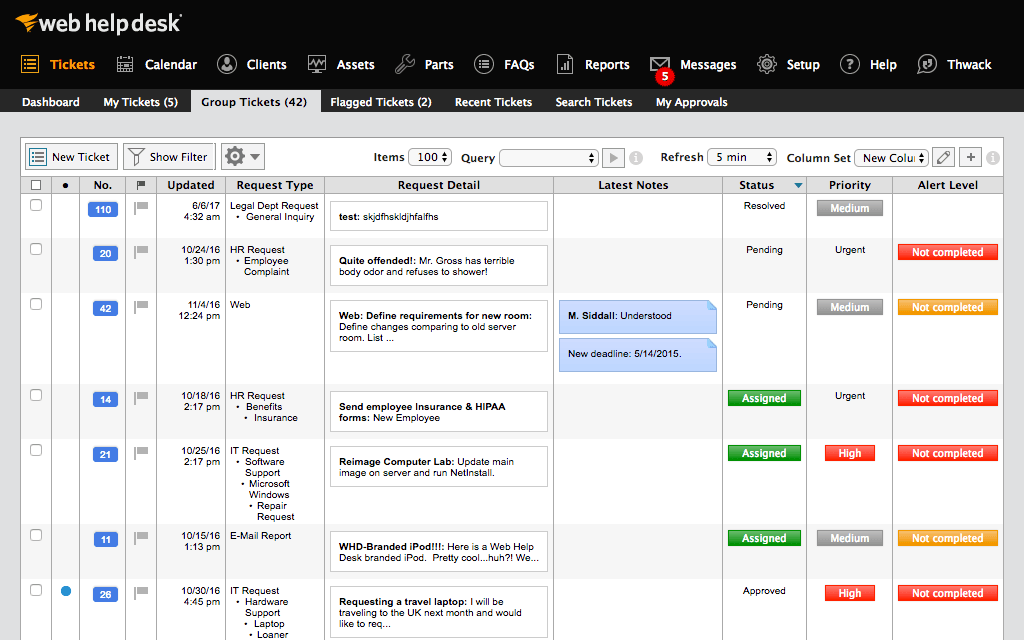
\includegraphics[height=6.8cm]{web-help-desk}
		\caption{Web Help Desk - piattaforma di \textit{ticketing} utilizzata.\newline
		\textbf{Fonte: }\url{https://www.webhelpdesk.com/}}
	\end{center}
\end{figure}

%**************************************************************
\subsection{Gestione della configurazione}

Per quanto riguarda la gestione della configurazione, tutti i progetti aziendali sono conservati in un \textit{repository} interno, completi di documentazione. \\
Anche il materiale prodotto durante lo stage è stato versionato, in modo da prevenire eventuali perdite di dati e permettere il ripristino in qualsiasi momento di una versione precedente.

%**************************************************************

\subsubsection{Strumenti di supporto}
Si fa affidamento a \textit{Git}, uno strumento di controllo versione distribuito. In particolare viene utilizzato \textit{Github}, servizio di \textit{hosting} che implementa \textit{Git} e facilita lo sviluppo di \textit{software} collaborativo.

%**************************************************************

\subsection{Sviluppo}

Per quanto riguarda l'attività di sviluppo, questa comprende: 
\begin{itemize}
	\item sviluppo di nuovi \textit{software}; 
	\item programmazione generica e modifiche su applicativi esistenti.
\end{itemize}
Gran parte degli applicativi utilizzati in azienda sono stati sviluppati internamente.\\
Prima di iniziare lo sviluppo di un nuovo software, si opera una raccolta dei requisiti attraverso un'analisi preliminare effettuata con i \textit{process owner} delle attività aziendali coinvolte e con gli utenti interni all'azienda che utilizzeranno il \textit{software}, per comprendere le necessità da soddisfare e le problematiche da risolvere.\\
In seguito si esegue un breve studio di fattibilità, sulla base delle tecnologie da utilizzare e sull'impegno richiesto in termini di tempo.\\
Successivamente si sottopone il risultato dell'analisi e dello studio all'\textit{IT Manager} e al \textit{CIO}. Una volta ricevuta l'approvazione, si procede con lo sviluppo.\\ 
Per quanto riguarda le richieste di programmazione generica come lo sviluppo di \textit{query} per estrazioni dal database, la progettazione di cruscotti per la \textit{BI}, modifiche ad alcune funzionalità nel gestionale, sviluppo di \textit{web service} per applicativi terzi o modifiche di piccola entità ad applicativi esistenti, gli sviluppatori riescono a gestire le richieste in autonomia con la sola supervisione dell'\textit{IT Manager}.


%**************************************************************

\subsubsection{Strumenti di supporto}
\begin{itemize}
	\item \textbf{Ambiente di sviluppo}: l'ambiente utilizzato per lo sviluppo degli applicativi è \textit{Visual Studio}, perché dispone di diversi \textit{template} per ciascun linguaggio di programmazione supportato, ad esempio applicazioni \textit{desktop}, libreria di classi, servizi di \textit{Windows}. Permette di sviluppare per piattaforme come \textit{Microsoft Azure}, della quale si utilizza in azienda il relativo servizio di \textit{Active Directory Azure AD}, per la gestione delle identità e l'autenticazione degli utenti;
	\item \textbf{Back-end}: i principali linguaggi utilizzati per lo sviluppo di nuovi \textit{software} sono \textit{C\#} e \textit{Java}. 
	Per quanto riguarda la persistenza dei dati è utilizzato principalmente \textit{SQL Server}.
	\item \textbf{Front-end}: viene adottato principalmente il \textit{framework Bootstrap}, perché semplifica la creazione di siti ed applicazioni \textit{web}, oltre a supportare il \textit{responsive web design}, permettendo che il \textit{layout} delle pagine \textit{web} si regoli dinamicamente, essendoci la necessità di rendere gli applicativi fruibili sia da \textit{desktop} che da dispositivi \textit{tablet} presenti nei reparti di produzione.
	\item \textbf{Programmazione \textit{BI}}: viene utilizzato \textit{Qlik Sense}, una piattaforma di \textit{data analytics}, che permette di creare soluzioni personalizzate per la \textit{BI} attraverso le \textit{API} messe a disposizione.
\end{itemize}



\begin{figure}[htbp]
	\begin{center}
		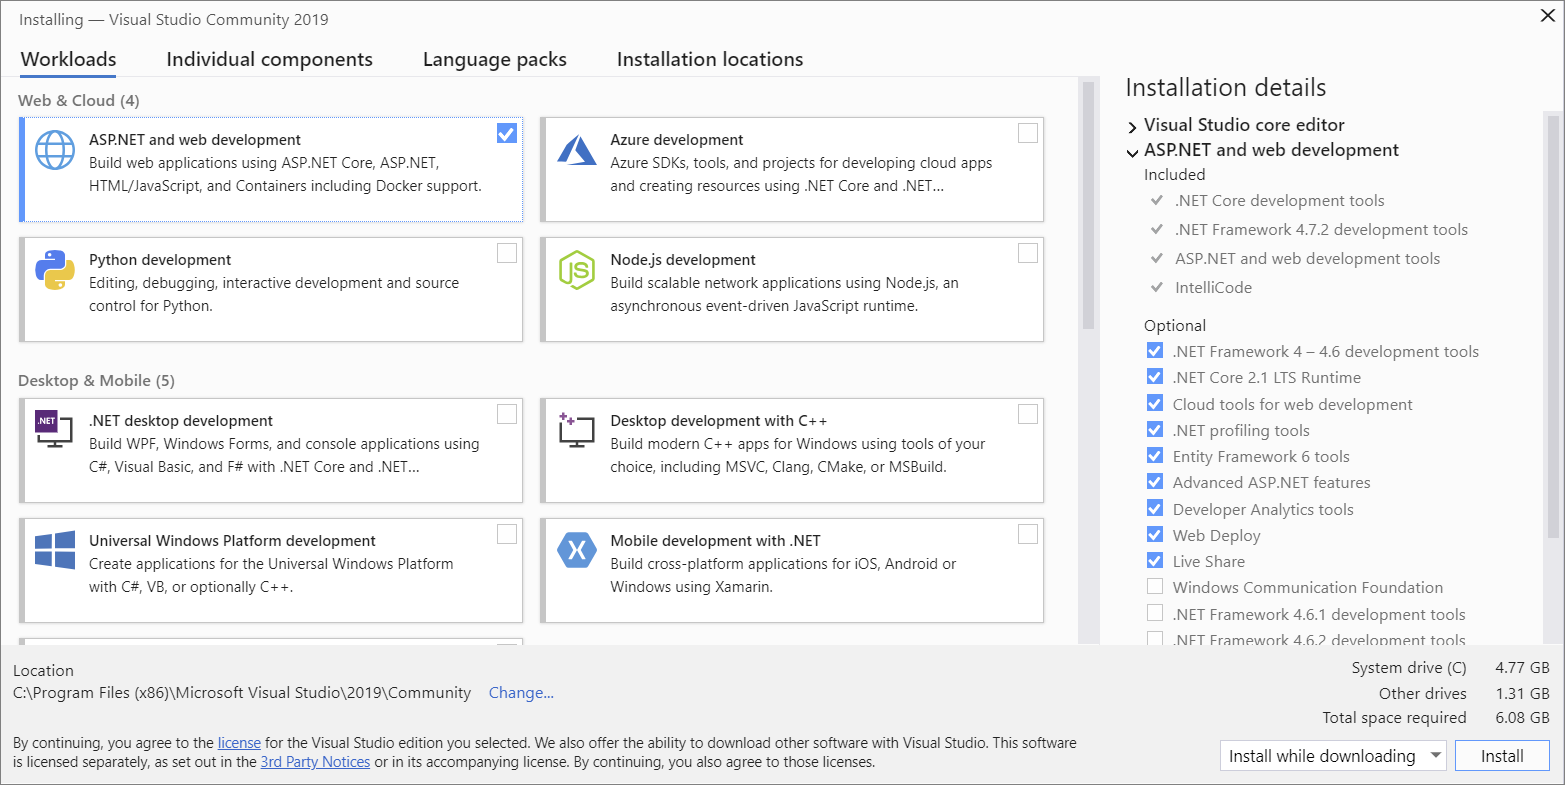
\includegraphics[height=5.9cm]{workloads-vs}
		\caption{Esempi di \textit{workloads} supportati da Visual Studio 2019. \newline
		\textbf{Fonte: } \url{https://visualstudio.microsoft.com}}
	\end{center}
\end{figure}


%**************************************************************

\subsection{Manutenzione}
 
 \subsubsection{Manutenzione del software}
Una volta terminato lo sviluppo di un prodotto \textit{software}, viene effettuato un rilascio in un ambiente di \textit{test} per un periodo di due settimane. Vengono effettuati \textit{test} che mettono in luce eventuali difetti del prodotto, in termini di usabilità e prestazioni, in modo da poterli correggere. Successivamente, avviene il rilascio ufficiale in produzione.\\
Viene svolta per tutta la vita del \textit{software} l'attività di manutenzione applicando correzioni dove necessario, riadattandolo sulla base dei cambiamenti dell'ambiente di produzione e aggiungendo nuove funzionalità in base alle esigenze degli utenti che lo utilizzano e dei processi che supportano.
 
 \subsubsection{Manutenzione sistemistica}
Sono gestiti internamente tutti gli aspetti di natura sistemistica, con il supporto di aziende esterne soprattutto nell'ambito della sicurezza informatica e nella gestione dell' infrastruttura.\\ Tutti i membri dell'\textit{IT} sono infatti formati in modo tale da supportare i tecnici esterni negli interventi che svolgono sull'infrastruttura aziendale. Le attività principali sono:
\begin{itemize}
	\item gestione dei \textit{server} virtuali;
	\item gestione degli apparati di rete (\textit{firewall}, \textit{switch}, \textit{router}, \textit{access point});
	\item gestione dei \textit{NAS}, \textit{Network Attached Storage}.
\end{itemize}

\subsubsection{Strumenti di supporto}
Per quanto riguarda la gestione dei \textit{server} virtuali, si fa affidamento a \textit{VMware vSphere}, una piattaforma di \textit{cloud computing} per la virtualizzazione.\\ Questa piattaforma permette di creare più sistemi di computer virtuali, chiamati macchine virtuali (\textit{VM}), che vengono eseguite su uno stesso \textit{server} fisico, chiamato \textit{host}).\\ Attraverso una pagina \textit{web} è possibile collegarsi al \textit{client web} \textit{vSphere Web Client} e gestire le \textit{VM} tramite le funzionalità messe a disposizione dall'interfaccia.


\begin{figure}[htbp]
	\begin{center}
		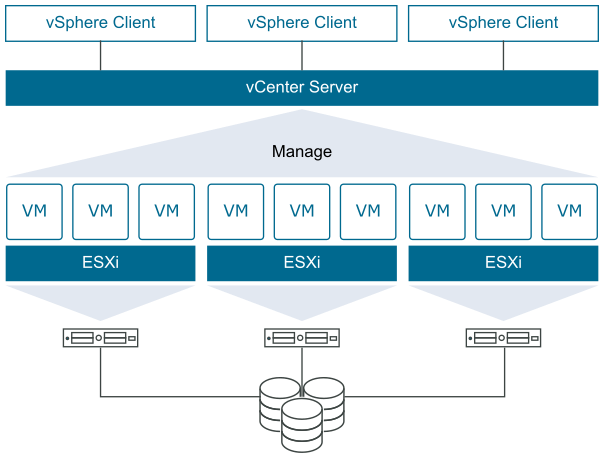
\includegraphics[height=5.5cm]{vsphere-2}
		\caption{Sintesi del servizio di virtualizzazione offerto da \textit{VMware vSphere}. \newline \textbf{Fonte: } \url{https://docs.vmware.com}}
	\end{center}
\end{figure}


\textit{Fortinet} è il \textit{firewall} adottato dall'azienda. La sua gestione avviene attraverso l'interfaccia \textit{web} di amministrazione, che permette di gestire gli utenti abilitati all'accesso alla rete aziendale tramite \textit{VPN}, le \textit{policy} che regolano il protocollo IPv4, il monitoraggio dell'attività di rete e gli apparati collegati (\textit{switch} e \textit{access point}).

\vspace{10pt}
\begin{figure}[htbp]
	\begin{center}
		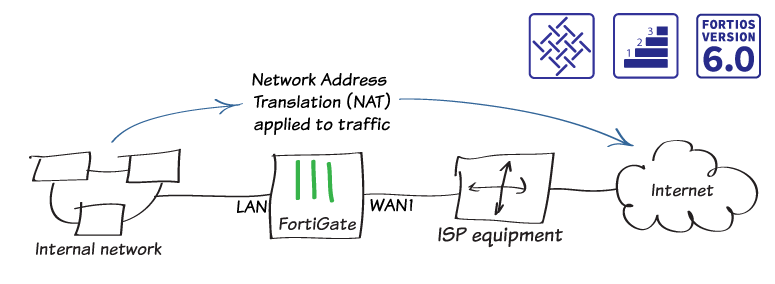
\includegraphics[height=4.5cm]{fortigate}
		\caption{Diagramma dell'implementazione di un sistema \textit{Fortigate} in modalità \textit{NAT}. \newline \textbf{Fonte: } \url{https://docs.fortinet.com}}
	\end{center}
\end{figure}
\vspace{10pt}

%**************************************************************

\section{Propensione all'innovazione}

L'azienda si impegna nella ricerca di nuovi strumenti e processi che permettano di migliorare il modo di lavorare portando beneficio ai dipendenti e all'azienda stessa.\\
Questo si manifesta attraverso l'investimento in corsi di formazione per migliorare lo \textit{smart working}, l'introduzione di applicativi come \textit{Microsoft Teams} per incrementare l'efficienza del lavoro di gruppo e l'implementazione di un sistema di comunicazione \textit{VOIP} che permette ai dipendenti l'utilizzo del telefono dell'ufficio attraverso un dispositivo personale mentre sono in \textit{smart working}. \\
Non sono state prese iniziative solamente per reagire alle necessità della situazione che stiamo vivendo, infatti l'azienda si sta dirigendo sempre di più verso una gestione \textit{cloud} dei servizi e all'utilizzo esteso di \textit{Microsoft Office 365} e di \textit{Sharepoint Online}, una soluzione per la collaborazione e la condivisione di documenti e informazioni, che è andata a sostituire quasi completamente l'archiviazione sui \textit{NAS} utilizzata finora.


%**************************************************************



%\section{Organizzazione del testo}

%\begin{description}
%    \item[{\hyperref[cap:processi-metodologie]{Il secondo capitolo}}] descrive %...
%    
%    \item[{\hyperref[cap:descrizione-stage]{Il terzo capitolo}}] approfondisce %...
%    
%    \item[{\hyperref[cap:analisi-requisiti]{Il quarto capitolo}}] %approfondisce ...
%    
%    \item[{\hyperref[cap:progettazione-codifica]{Il quinto capitolo}}] %approfondisce ...
%    
%    \item[{\hyperref[cap:verifica-validazione]{Il sesto capitolo}}] approfondisce ...
%    
%    \item[{\hyperref[cap:conclusioni]{Nel settimo capitolo}}] descrive ...
%\end{description}

%Riguardo la stesura del testo, relativamente al documento sono state adottate le seguenti convenzioni tipografiche:
%\begin{itemize}
%	\item gli acronimi, le abbreviazioni e i termini ambigui o di uso non comune menzionati vengono definiti nel glossario, situato alla fine del presente documento;
%	\item per la prima occorrenza dei termini riportati nel glossario viene utilizzata la seguente nomenclatura: \emph{parola}\glsfirstoccur;
%	\item i termini in lingua straniera o facenti parti del gergo tecnico sono evidenziati con il carattere \emph{corsivo}.
%\end{itemize}